
\pagebreak	
\section{Die Terminplanung benutzen}
\label{bkm:Ref445400921}
In der aktuellen CUBE PA Version haben Sie die Möglichkeit Terminpläne (bspw. als PDF) hochzuladen und den Projektmitarbeitern, welche CUBE PA benutzen, zugänglich zu machen. In vorliegender Dokumentation wurden beispielhaft zwei Terminpläne importiert und bereitgestellt: 'Gesamtterminprogramm' und 'Studienauftragsverfahren'. \\
Als zweite Funktion der Terminplanung können Sie komplexe Terminpläne, welche mit Microsoft Project erstellt wurden als .xml-File importieren und anschliessend in CUBE PA filtern und benutzerspezifische Ansichten generieren.

%Die Terminplanung beschränkt sich in dern aktuellen CUBE PA Version auf das Herunterladen des Gesamtterminprogramms und das Studienauftragsverfahren Bhf, sowie die Filterung und entsprechenden Anzeige des Detailterminprogramms.

\subsection{Die gewünschte Ansicht der Terminplanung}

\begin{wrapfigure}[8]{l}{6.5cm}   % [x] Wie manche Zeile soll sich um die Grafik "brechen"
  \vspace{-35pt}      % Grundwert war 20; mit 30 schön oben beim Text ausgerichtet
  \begin{center}
    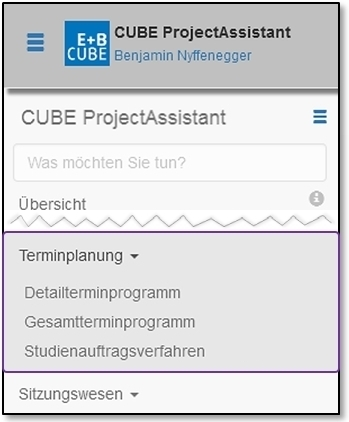
\includegraphics[width=1\linewidth]{../chapters/04_Terminplanung/pictures/4-1_Menu_Terminplanung.jpg}
  \end{center}
  \vspace{-20pt}
  \caption{Die Terminplanung verwenden}
  \vspace{-10pt}
\end{wrapfigure}

Wählen Sie aus dem Menü links den Punkt 'Terminplanung' und dann den gewünschten Unterpunkt. (Mit Klick auf 'Terminplanung' werden lediglich die Unterpunkte auf- und zugeklappt). Bei der Terminplanung haben Sie die Möglichkeit kundenspezifische Terminpläne hinzuzufügen. Entsprechend sieht das Menü unter Umständen bei Ihnen anders aus als in der Dokumentation.

\vspace{5cm} 

\subsection{Das Gesamtterminprogramm und das Studienauftragsverfahren}

Bei diesen beiden Funktionen handelt es sich um das Herunterladen des entsprechenden Terminprogramms.\newline
Wenn Sie im Menü unter Terminplan den Unterpunkt 'Gesamtterminprogramm' auswählen, erscheint folgende Ansicht (Diese Ansicht ist abhängig von der CUBE PA-Konfiguration):
% kundenspezifisch
\begin{figure}[H]
\center{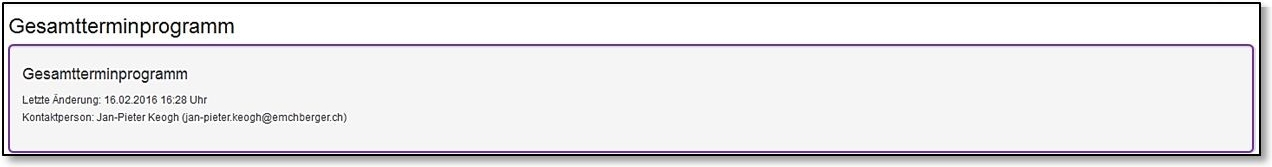
\includegraphics[width=1\linewidth]{../chapters/04_Terminplanung/pictures/4-2_Gesamtterminprogramm.jpg}}
\caption{Gesamtterminprogramm}
% \label{fig:speciation}
\end{figure}

Klicken Sie in den violett umrahmten Bereich, um das Gesamtterminprogramm herunterzuladen. Im nächsten Fenster können Sie wählen, ob das Dokument geöffnet werden soll oder ob Sie es an einem beliebigen Ort abspeichern wollen.

\vspace{\baselineskip}

Wenn Sie im Menü unter Terminplan den Unterpunkt 'Studienauftragsverfahren Bhf' auswählen, erscheint folgende Ansicht:

% kundenspezifisch
\begin{figure}[H]
\center{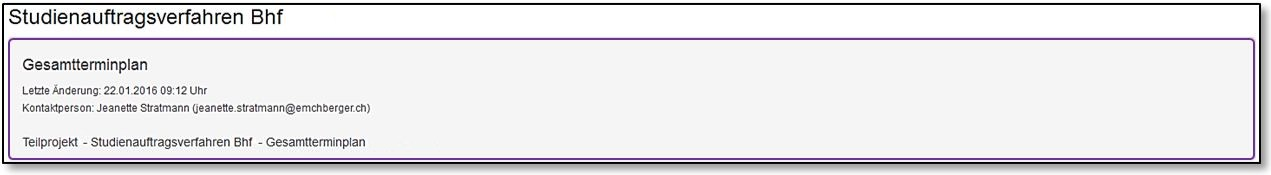
\includegraphics[width=1\linewidth]{../chapters/04_Terminplanung/pictures/4-2_Studienauftragsv.jpg}}
\caption{Studienauftragsverfahren Bhf}
% \label{fig:speciation}
\end{figure}

Klicken Sie in den violett umrahmten Bereich, um das Studienauftragsverfahren Bhf herunterzuladen. Im nächsten Fenster können Sie wählen, ob das Dokument geöffnet werden soll oder ob Sie es an einem beliebigen Ort abspeichern wollen.

\subsection{Das Detailterminprogramm}

Wählen Sie im Menü unter Terminplan den Unterpunkt 'Detailterminprogramm'. Es erscheint folgendes Fenster, in welchem Sie die gewünschten Filtereinstellungen vornehmen können:

\begin{figure}[H]
\center{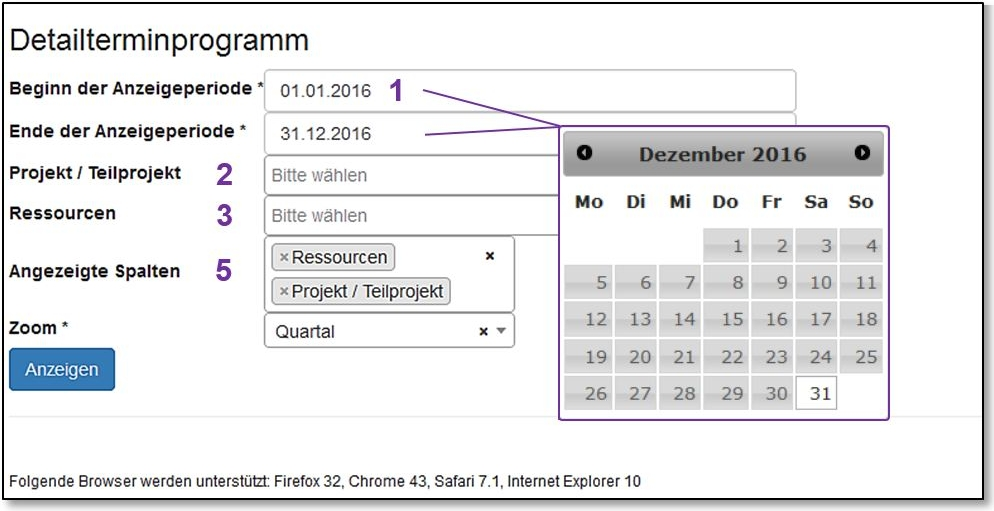
\includegraphics[width=.75\linewidth]{../chapters/04_Terminplanung/pictures/4-3_Detailterminprogramm.jpg}}
\caption{Detailterminprogramm}
% \label{fig:speciation}
\end{figure}

Die Felder mit einem * sind Pflichtfelder und müssen ausgewählt werden. Wählen Sie den Beginn und das Ende der Anzeigeperiode \col{(1)}. Es erscheint eine Kalenderansicht, mit welcher Sie das gewünschte Datum auswählen. Sie können fakultativ ein Projekt / Teilprojekt \col{(2)} und ebenso Ressourcen \col{(3)} auswählen.

\begin{figure}[H]
\center{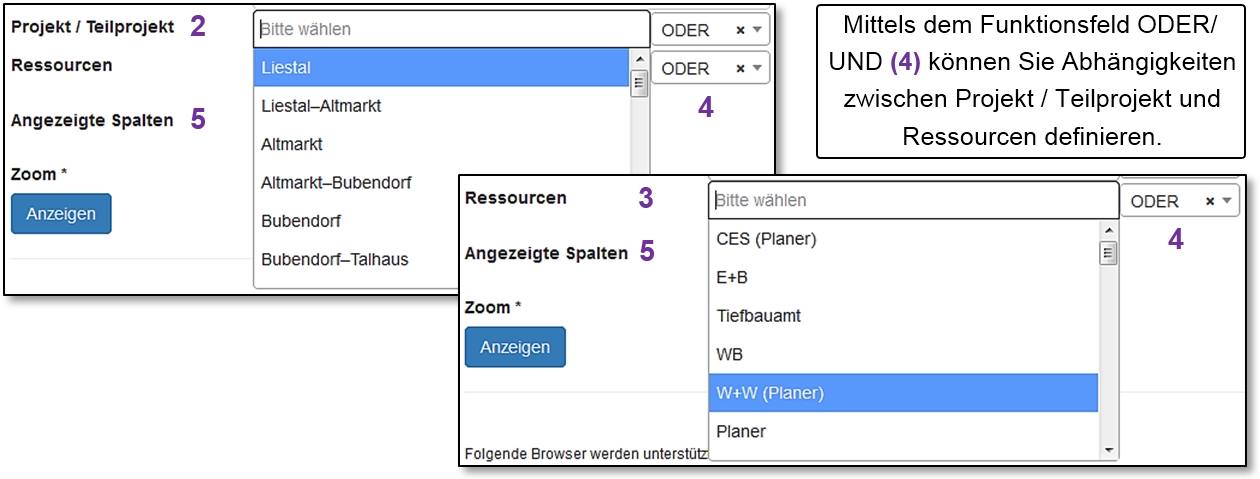
\includegraphics[width=1\linewidth]{../chapters/04_Terminplanung/pictures/4-3_Termine_Abhaengigkeiten.jpg}}
\caption{Abhängigkeiten definieren}
% \label{fig:speciation}
\end{figure}

% Text als Grafik implementiert
% Mittels dem Funktionsfeld ODER/UND \textbf{\textcolor[rgb]{0.4392157,0.1882353,0.627451}{(4)}} können Sie Abhängigkeiten zwischen Projekt / Teilprojekt und Ressourcen definieren.

Wählen Sie, welche Spalten (Projekt / Teilprojekt, Ressourcen) im Filterergebnis angezeigt werden sollen \col{(5)}. Durch erneutes Klicken in das Feld 'Angezeigte Spalte' können Sie auch eine zweite Spalte auswählen. Um nach Projekt / Teilprojekt oder Ressourcen zu filtern und die Spalten im Terminplan anzeigen zu können, müssen im MS Project File die entsprechenden Informationen vorhanden sein (siehe Kapitel \ref{bkm:Ref445411998}).

% Ref einfügen nach 12.1

\vspace{\baselineskip}

\begin{wrapfigure}[4]{r}{6cm}
  \vspace{-30pt}
  \begin{center}
    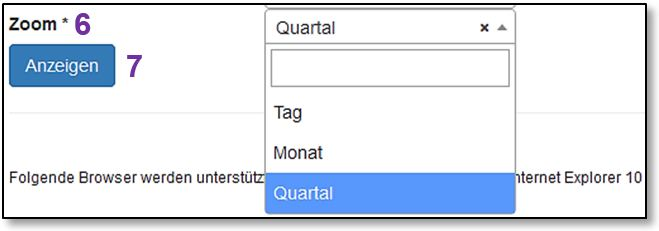
\includegraphics[height=25mm]{../chapters/04_Terminplanung/pictures/4-3_Zoom-Ansicht.jpg}
  \end{center}
  \vspace{-20pt}
  \caption{Zoom Ansicht}
  \vspace{-10pt}
\end{wrapfigure}
Unter Zoom \col{(6)} können Sie auswählen, ob Sie eine Tages-, Monats- oder Quartalsansicht wünschen. Wurden die gewünschten Filtereinstellungen vorgenommen klicken Sie auf 'Anzeigen' \col{(7)}.

\vspace{\baselineskip}
\vspace{\baselineskip}

Nach Klick auf 'Anzeigen' erhalten Sie das gefilterte Ergebnis des Terminkalenders:

\begin{figure}[H]
\center{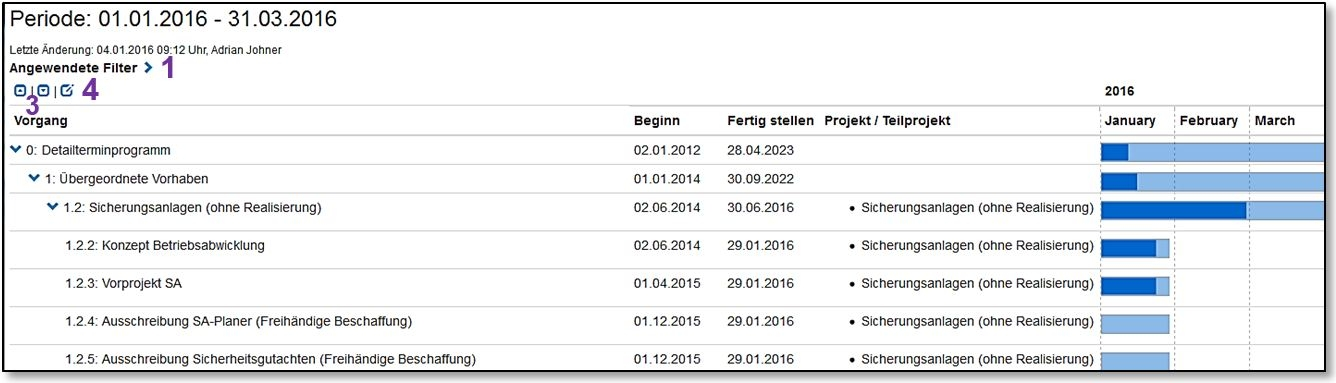
\includegraphics[width=1\linewidth]{../chapters/04_Terminplanung/pictures/4-3_Termin_Ergebnis.jpg}}
\caption{Ergebnis des Terminkalenders}
% \label{fig:speciation}
\end{figure}

Durch Klick auf die Klammer 
\includegraphics[height=12pt]{/Icons/Pfeil_rechts.jpg} \col{(1)} können Sie sich den angewendeten Filter anzeigen lassen. Durch erneuten Klick auf die Klammer 
\includegraphics[height=12pt]{/Icons/Pfeil_unten.jpg} \col{(2)} wird die Ansicht eingeklappt.

\begin{figure}[H]
\center{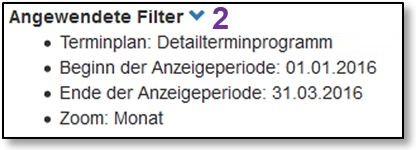
\includegraphics[width=.4\linewidth]{../chapters/04_Terminplanung/pictures/4-3_Termin_Filter.jpg}}
\caption{Angewendete Filter}
% \label{fig:speciation}
\end{figure}

Mit den beiden Pfeilen 
\includegraphics[height=12pt]{/Icons/Pfeil_auf-ab.jpg} \col{(3)} lassen sich alle Details anzeigen, respektive ausblenden. Soll der Filter erneut angepasst werden, klicken Sie auf das Bearbeitungssymbol 
\includegraphics[height=12pt]{/Icons/Bearbeiten.jpg} \col{(4)}.
